% !TEX root = dissertation_BB.tex
%% spellcheck-language en-US

%    #
%   #
%  #  #
%  #####
%     #

\chapter{Real-time, GPU accelerated image processing pipeline}

\graphicspath{{./figures/4_gpu/}}


\section{GPU architecture}

\section{Live fusion}
  \subsection{MuVi-SPIM}
  \subsection{Bead based registration}

\section{B³D image compression}
  \b3d image compression
  B³D image compression

  \subsection{Data sizes in microscopy}

    \begin{figure}[tpb]
      \centering
      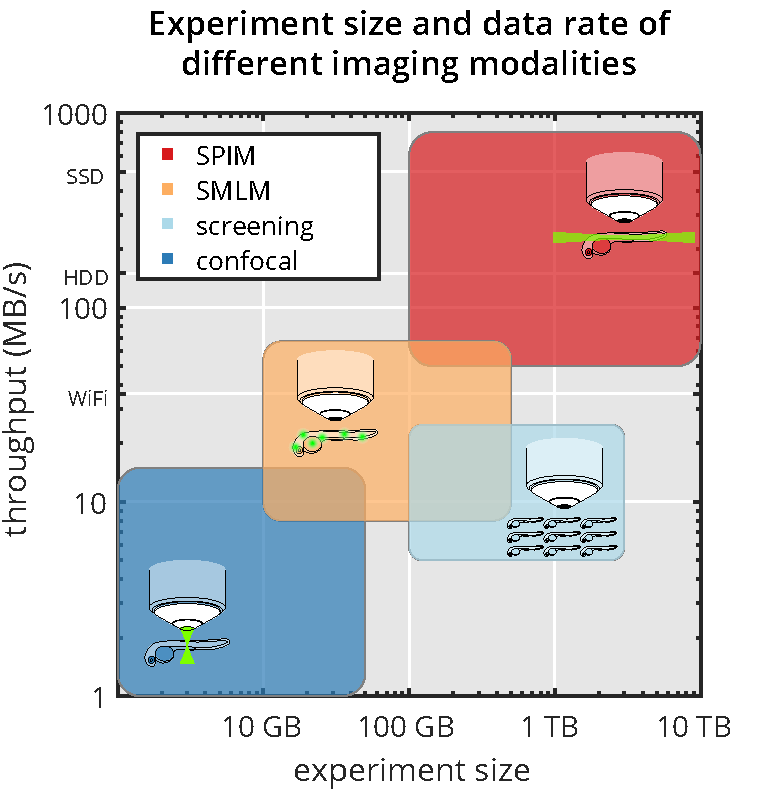
\includegraphics[page=1,width=0.5\textwidth]{comparison_with_pictograms}
      \bcaption[Experiment sizes and data rate of different imaging modalities]{Comparison of single-plane illumination microscopy (SPIM, red rectangle), high-content screening (light blue), single molecule localization microscopy (SMLM, orange) and confocal microscopy (blue) by typical experiment size and data production rate (see also Table \ref{tab:sizes}).}
      \label{fig:sizes}
    \end{figure}


    

  \subsection{Compression algorithm}

    \begin{figure}[tpb]
      \centering
      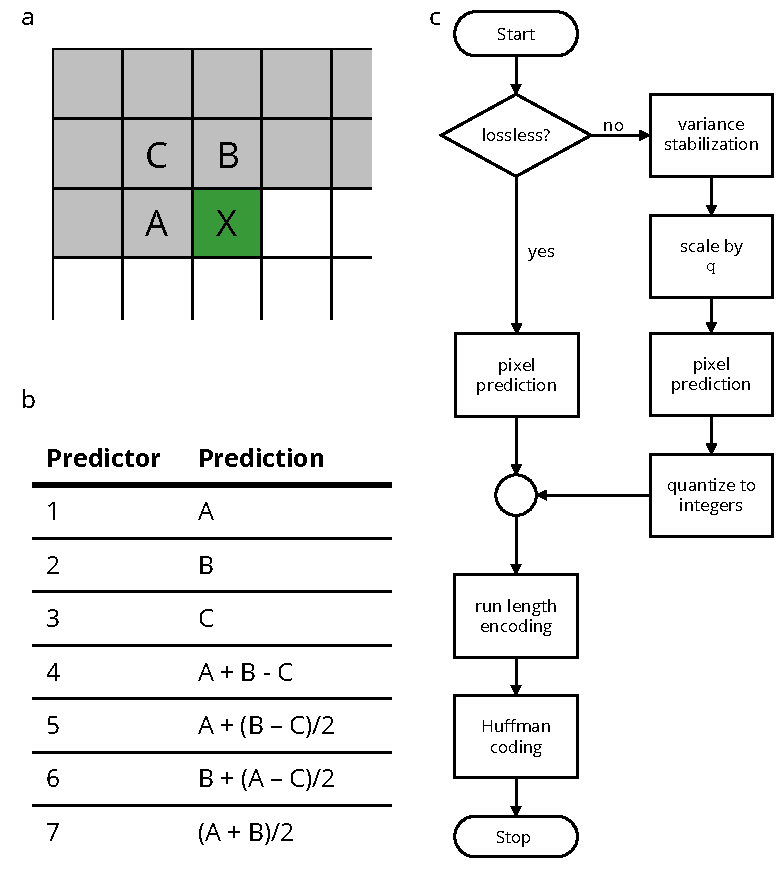
\includegraphics[page=1,width=0.6\textwidth]{SFig1_flow}
      \bcaption[\b3d algorithm schematics]{(\textbf{a}) Prediction context for pixel X, the next sample to be encoded. Three neighboring pixels are considered: left (A), top (B) and top left (C) neighbors. (\textbf{b}) Lossless JPEG predictors for X, based on the context showed in (\textbf{a}). The first three predictors are one-dimensional, while the rest are two-dimensional. Using a two dimensional predictor while increases complexity slightly, also increases the achievable compression ratio. We found that for fluorescence microscopy images predictor 7 performs best, hence its inclusion in the \b3d algorithm. (\textbf{c)} Complete algorithm flowchart depicting the main stages of the compression. First, if the result should be lossless, pixel prediction is performed on the original image values. If within noise level mode is selected, the image noise is stabilized first (see "\textbf{Supplementary Note}"), which is then scaled by the quantization step q. Prediction is performed, and the prediction errors are rounded to the nearest integer. The prediction errors for both lossless and lossy modes are then run-length encoded, and finally Huffman coding is applied to effectively reduce data size. The output of the Huffman coder is saved as the compressed file.}
      \label{fig:algorithm}
    \end{figure}


  \subsection{Lossless compression performance}

    \begin{figure}[tpb]
      \centering
      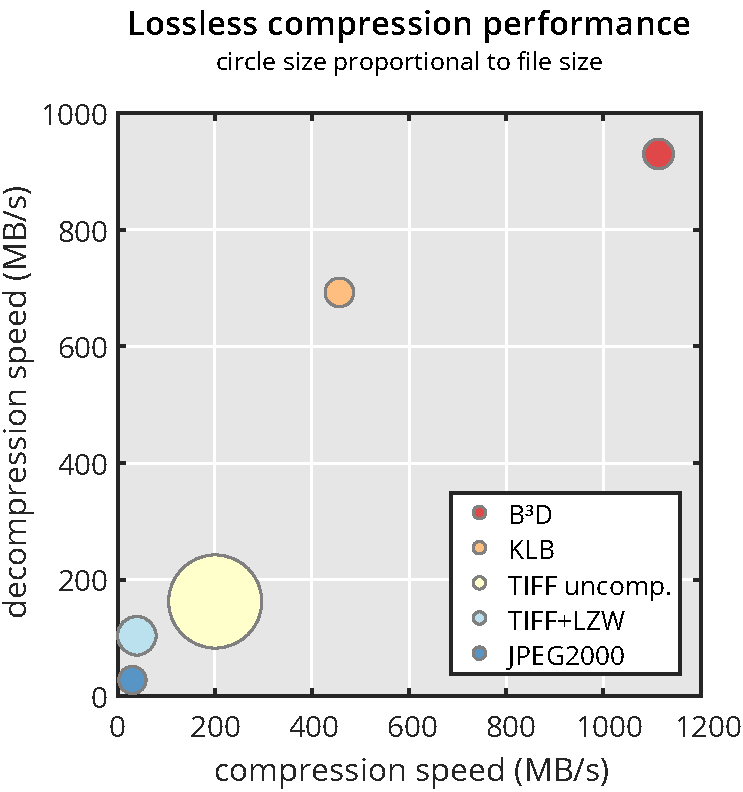
\includegraphics[page=1,height=0.5\textwidth]{bubbles}
      \bcaption[Lossless compression performance]{Performance comparison of our B³D \b3d compression algorithm (red circle) vs. KLB (orange), uncompressed TIFF (light yellow), LZW compressed TIFF (light blue) and JPEG2000 (blue) regarding write speed (horizontal axis), read speed (vertical axis) and file size (circle size). (see also Table \ref{tab:performance}).}
      \label{fig:performance}
    \end{figure}

    


  \subsection{Swapping for WNL}

    \begin{figure}[tpb]
      \centering
      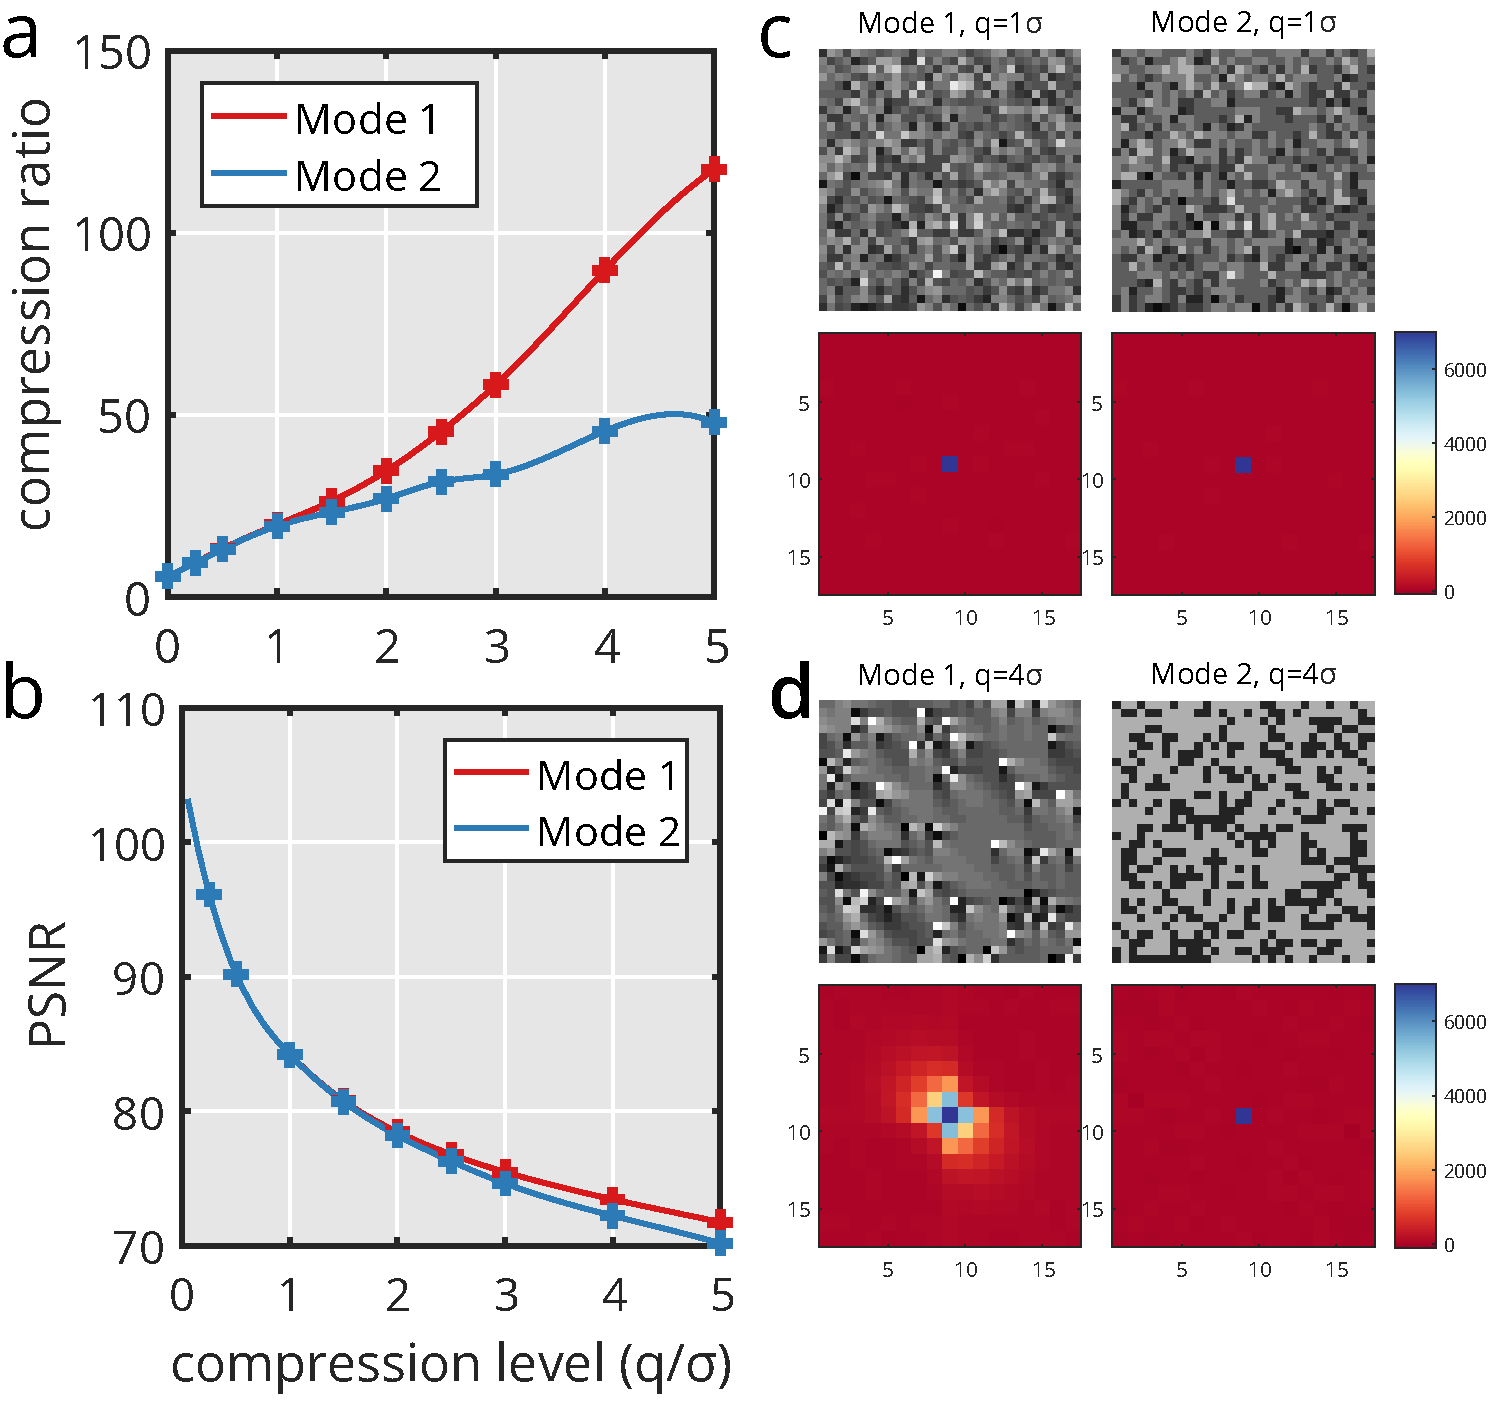
\includegraphics[page=1,width=0.7\textwidth]{swapping}
      \bcaption[Options for noise dependent lossy compression]{Comparing Mode 1 (prediction then quantization) and Mode 2 (quantization then prediction) of noise dependent lossy compression in terms of compression ratio, peak signal to noise ratio (PSNR) and spatial correlations introduced to random noise. (\textbf{a}) Compression ratio as a function of the quantization step for Mode 1 and Mode 2. (\textbf{b}) PSNR as a function of the quantization step for Mode 1 and Mode 2. (\textbf{c, d}) Random noise was compressed at various quantization steps both for Mode 1 and Mode 2. Autocorrelation was calculated for the compressed images to see whether the compression introduces any spatial correlation between the pixels. For q=1$\upsigma$ both modes are free of correlation (\textbf{c}, top: compressed images, bottom: autocorrelation), however, for q=2$\upsigma$ Mode 1 exhibits a correlation pattern (\textbf{d}, top left: compressed image, bottom left: autocorrelation) that is not present in Mode 2 (\textbf{d}, top right compressed image, bottom right: autocorrelation). For more discussion, see "\textbf{Supplementary Note}".}
      \label{fig:swapping}
    \end{figure}

  \subsection{Benchmarking}

    \begin{figure}[tpb]
      \centering
      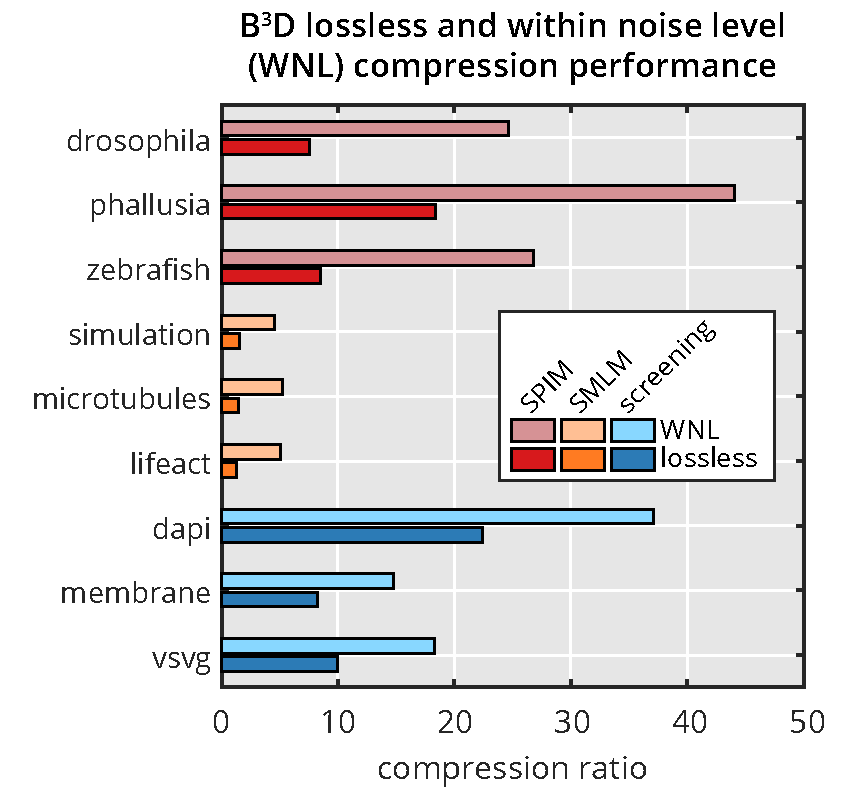
\includegraphics[page=1,height=0.5\textwidth]{Fig1c_compressionBars}
      \bcaption[Within noise level compression performance]{WNL compression performance compared with lossless performance for 9 different dataset representing 3 imaging modalities (SPIM, SMLM, screening). Compression ratio = original size / compressed size. For description of datasets see Table \ref{tab:datasets} in Appendix B.}
      \label{fig:benchmark}
    \end{figure}

    \begin{figure}[tpb]
      \centering
      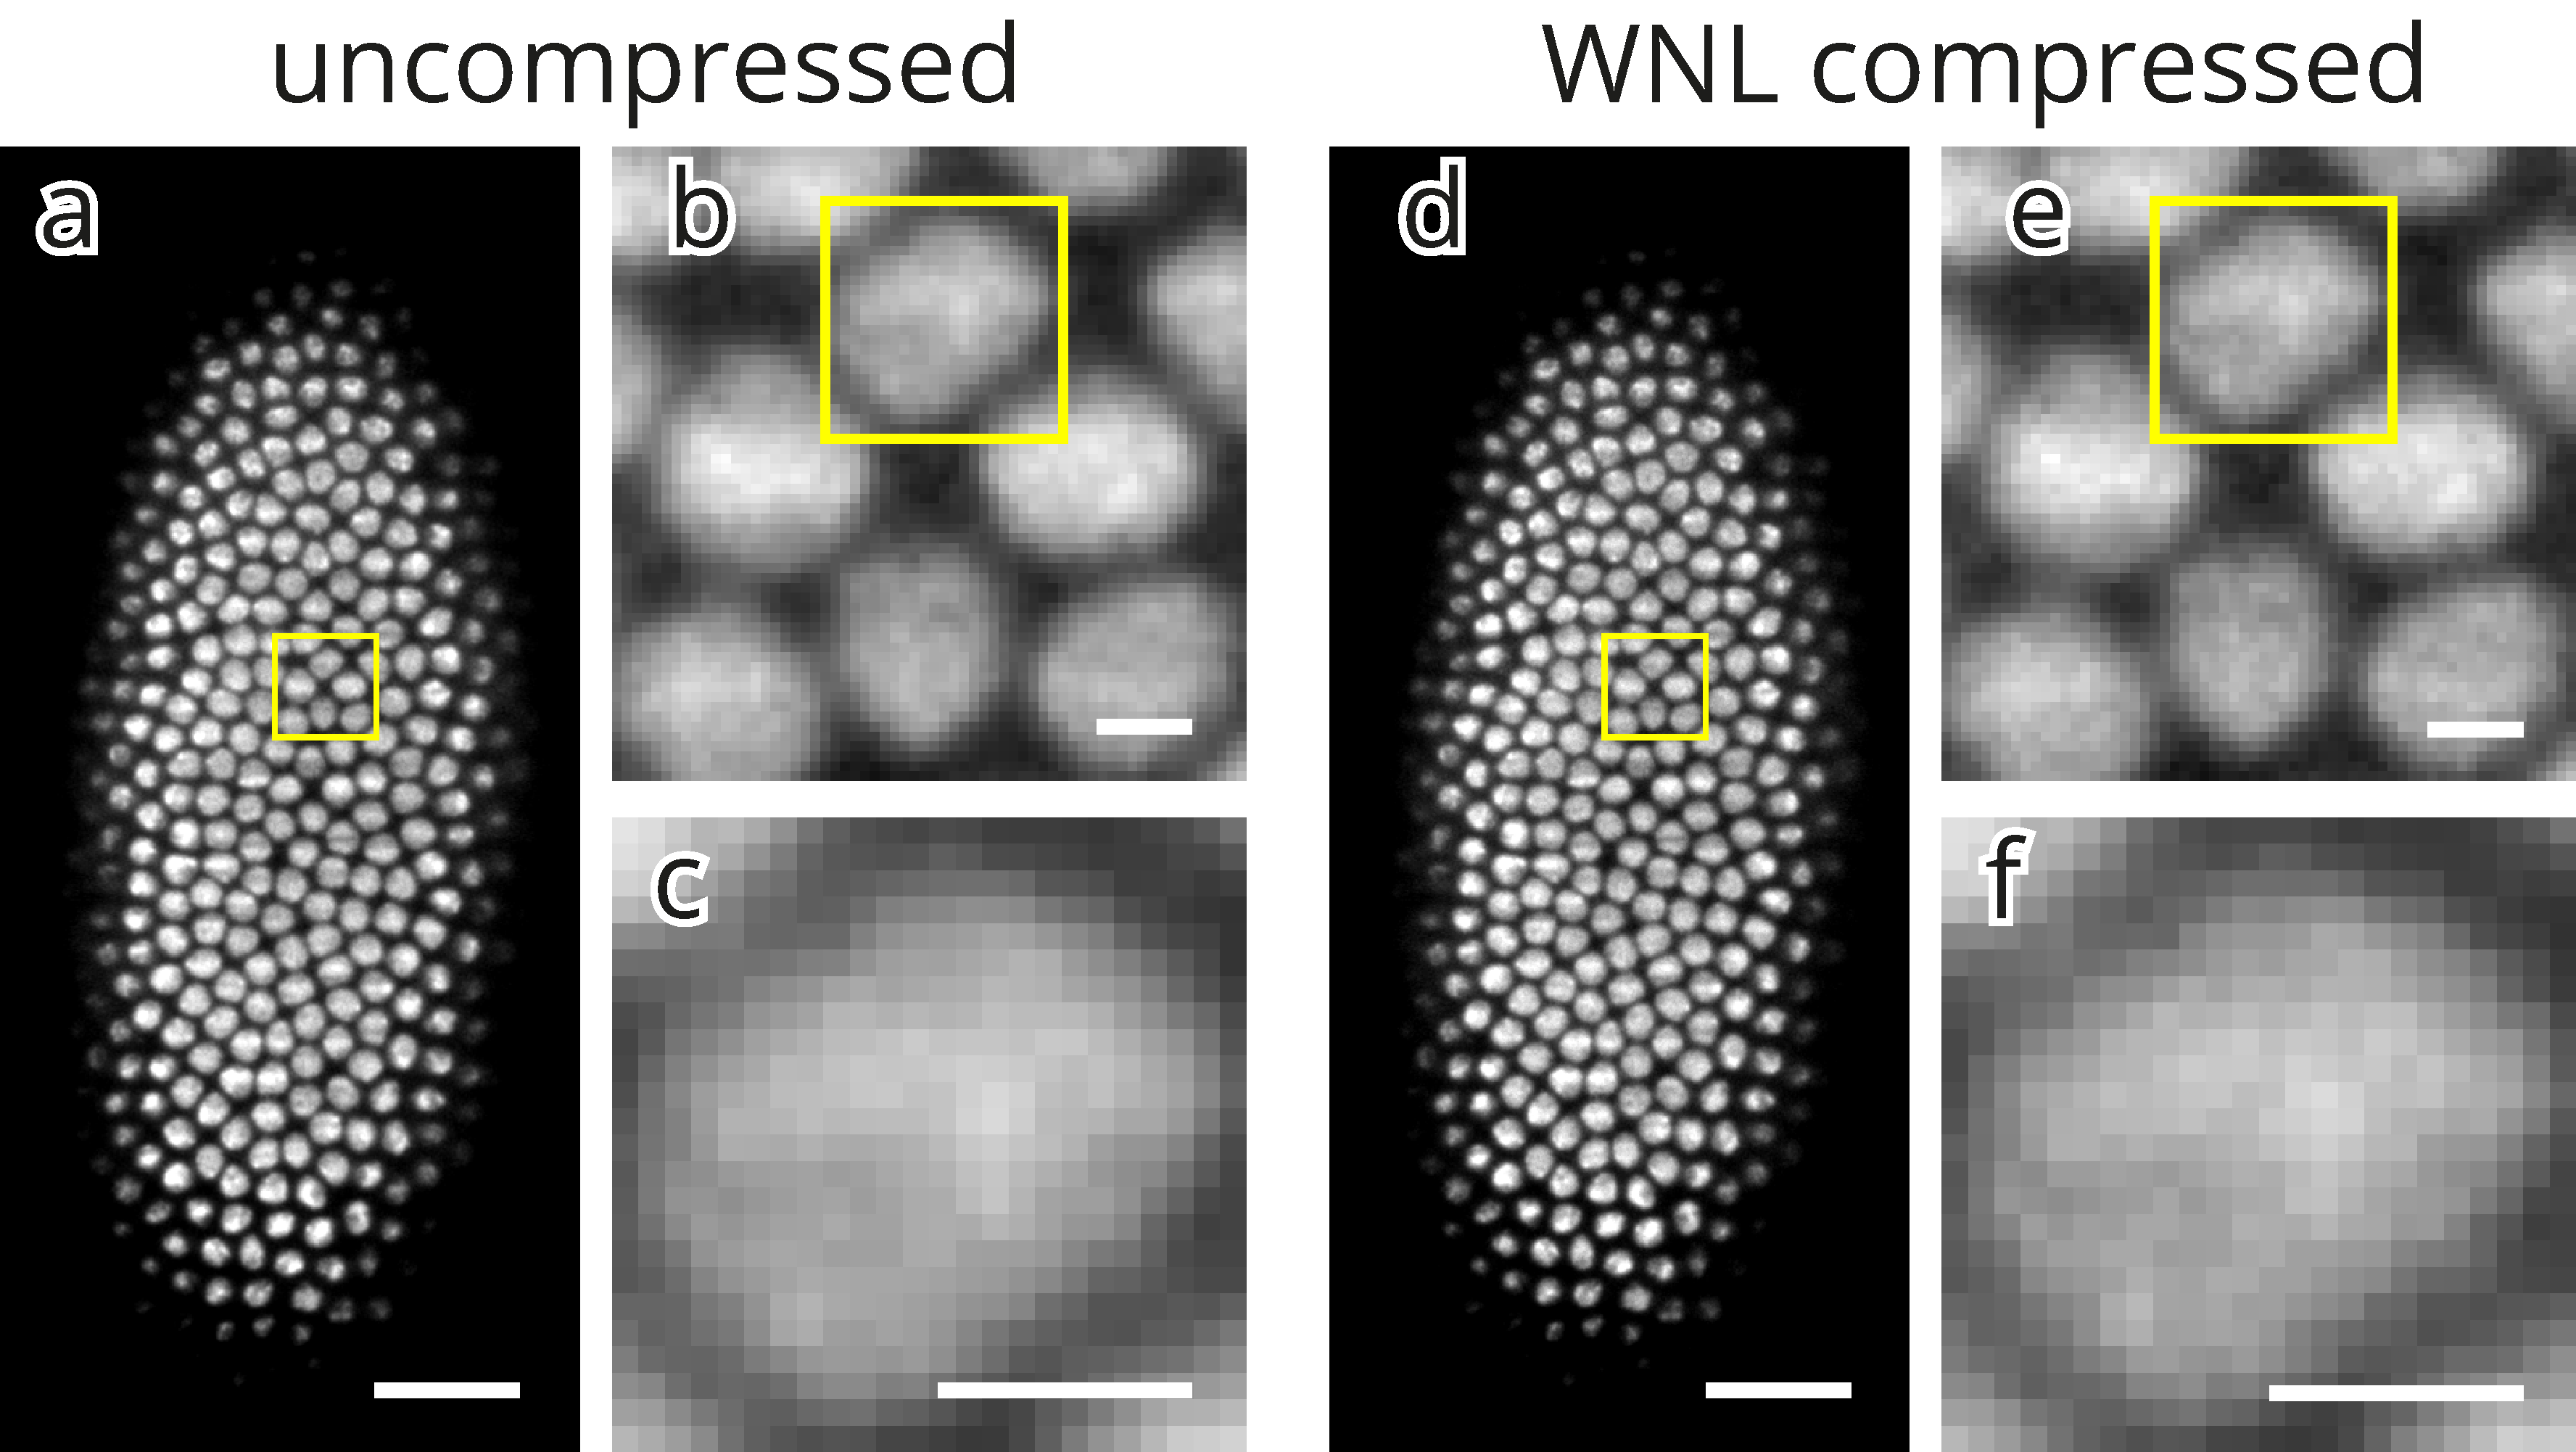
\includegraphics[page=1,width=0.9\textwidth]{wnlSamples}
      \bcaption[Image quality of a WNL compressed dataset]{WNL compression performance compared with lossless performance for 9 different dataset representing 3 imaging modalities (SPIM, SMLM, screening). Compression ratio = original size / compressed size. For description of datasets see Table \ref{tab:datasets}.}
      \label{fig:wnlSamples}
    \end{figure}

    \begin{figure}[tpb]
      \centering
      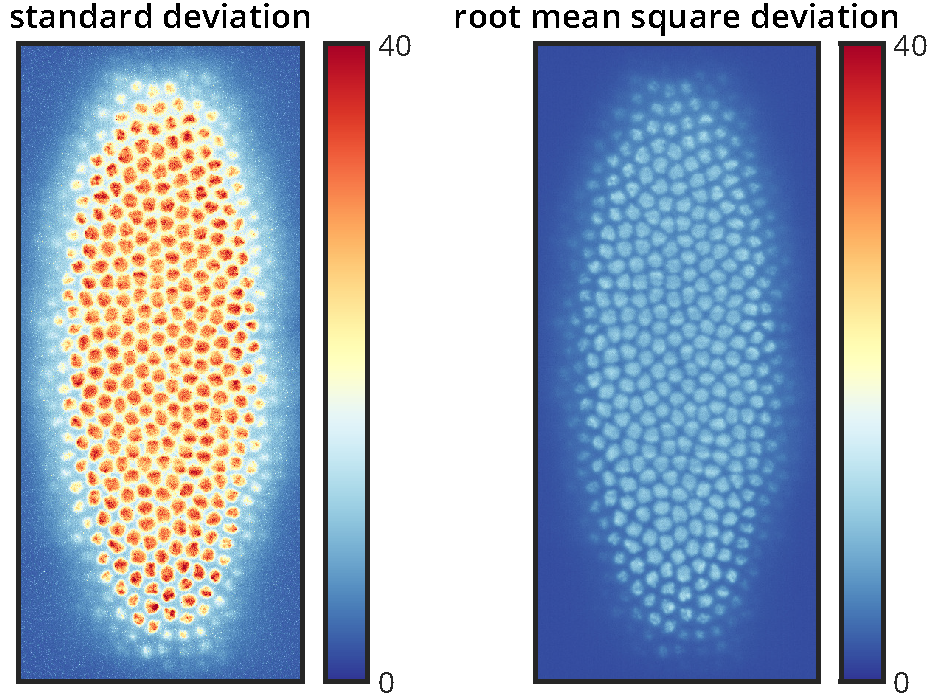
\includegraphics[page=1,width=0.7\textwidth]{SFig4_RMSDvsSD}
      \bcaption[Compression error compared to image noise]{To compare the difference arising from WNL compression to image noise, we imaged a single plane 100 times in a \textit{Drosophila melanogaster} embryo expressing H2Av-mCherry nuclear marker at \SI{38}{ms} intervals. The whole acquisition took \SI{3.8}{s}, for which the sample can be considered stationary. To visualize image noise, the standard deviation was calculated for the uncompressed images (left). All images were then WNL compressed, and the root mean square deviation was calculated compared to the uncompressed images (right). The root mean square deviation on average is 3.18 times smaller than the standard deviation of the uncompressed images.}
      \label{fig:RMSD}
    \end{figure}

    

    \begin{figure}[tpb]
      \centering
      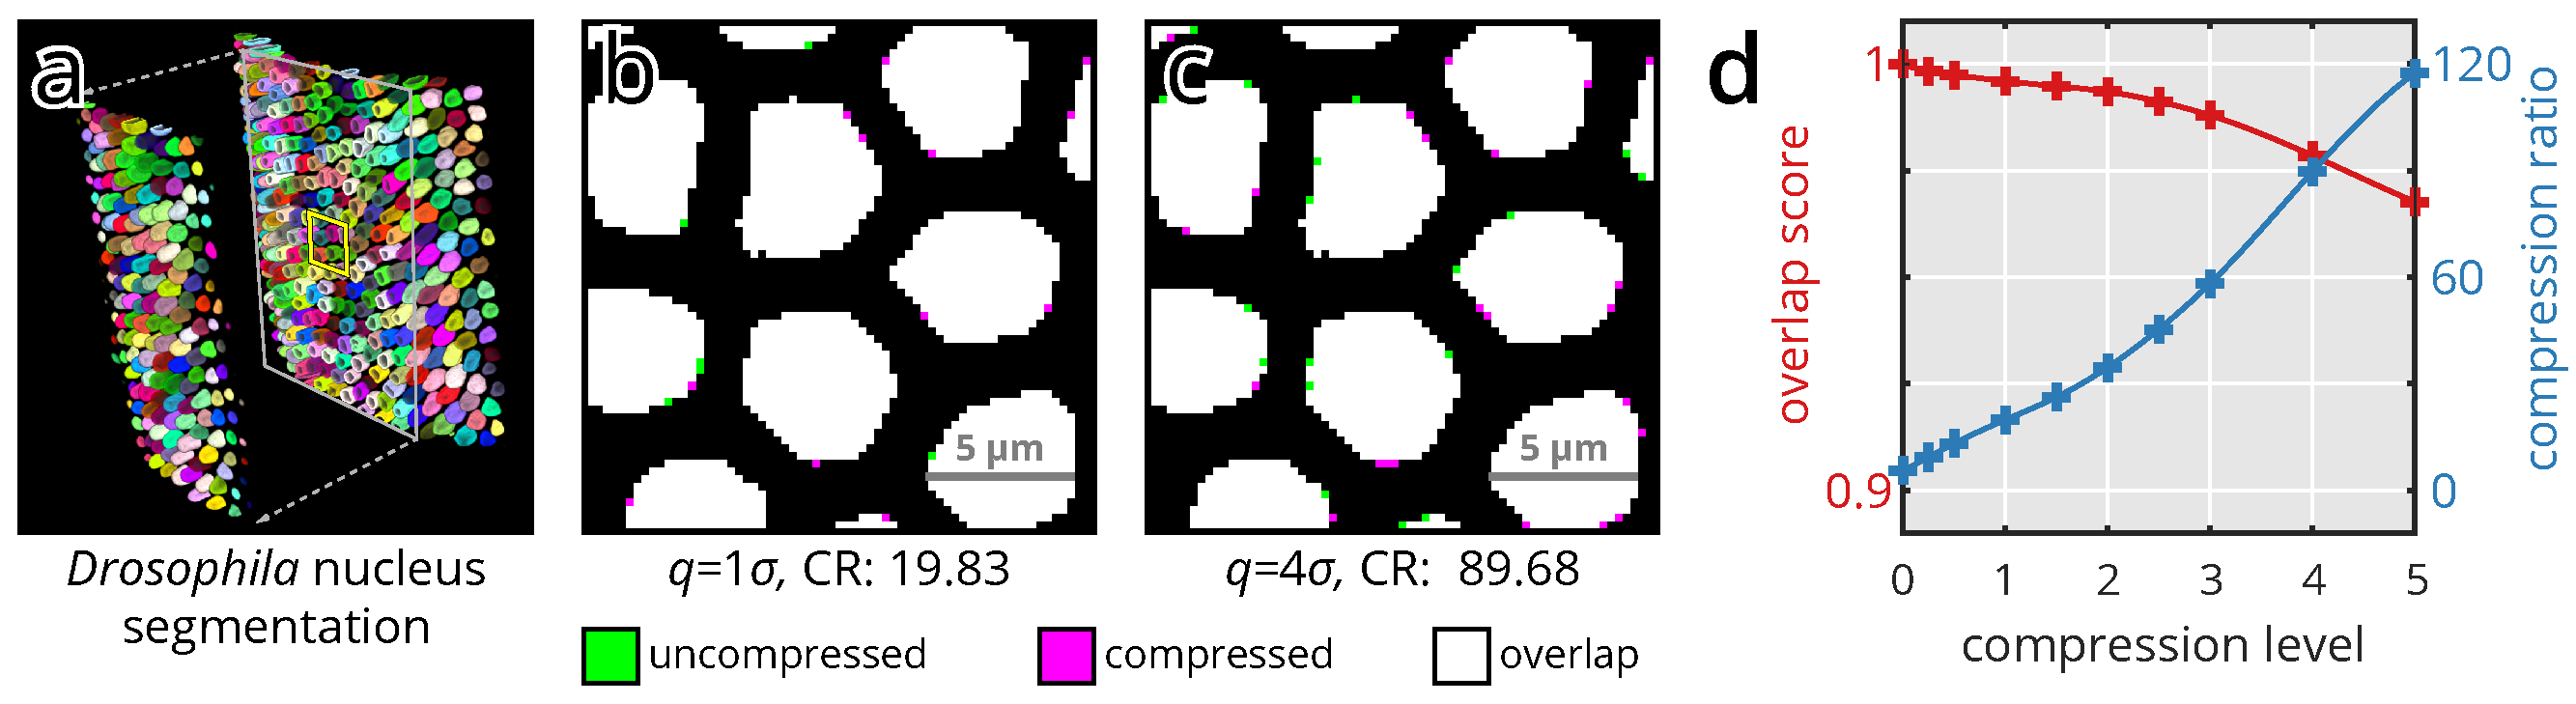
\includegraphics[page=1,width=1\textwidth]{LLvsB3D}
      \bcaption[Influence of noise dependent lossy compression on 3D nucleus segmentation]{A \textit{Drosophila melanogaster} embryo expressing H2Av-mCherry nuclear marker was imaged in MuVi-SPIM \cite{krzic_multiview_2012}, and 3D nucleus segmentation was performed ( "\textbf{Online Methods}") (\textbf{a}). The raw data was subsequently compressed at increasingly higher compression levels, and segmented based on the training of the uncompressed data. To visualize segmentation mismatch, the results of the uncompressed (green) and compressed (magenta) datasets are overlaid in a single image (\textbf{b}, \textbf{c}; overlap in white). Representative compression levels were chosen at two different multiples of the photon shot noise, at q=1$\upsigma$ (\textbf{b}) and q=4$\upsigma$ (\textbf{c}). For all compression levels the segmentation overlap score ( "\textbf{Online Methods}") was calculated and is plotted in (\textbf{g}) along with the achieved compression ratios.}
      \label{fig:wnlDroso}
    \end{figure}

    \begin{figure}[tpb]
      \centering
      \includegraphics[page=3,width=1\textwidth]{LLvsB3D}
      \bcaption[Influence of noise dependent lossy compression on 3D membrane segmentation]{A \textit{Phallusia mammillata} embryo expressing PH-citrine membrane marker was imaged in MuVi-SPIM \cite{krzic_multiview_2012}, and 3D membrane segmentation was performed ( "\textbf{Supplementary Methods}") (\textbf{a}). The raw data was subsequently compressed at increasingly higher compression levels, and segmented using the same settings as the uncompressed data. To visualize segmentation mismatch, the results of the uncompressed (green) and compressed (magenta) datasets are overlaid in a single image (\textbf{b, c}; overlap in white). Representative compression levels were chosen at two different multiples of the photon shot noise, at q=1.6$\upsigma$ (\textbf{b}) and q=4.8$\upsigma$ (\textbf{c}). For all compression levels the segmentation overlap score ( "\textbf{Supplementary Methods}") was calculated and is plotted in (\textbf{d}) along with the achieved compression ratios.}
      \label{fig:wnlPhallusia}
    \end{figure}

    \begin{figure}[tpb]
      \centering
      \includegraphics[page=2,width=1\textwidth]{LLvsB3D}
      \bcaption[Influence of noise dependent lossy compression on single-molecule localization]{Microtubules, immunolabeled with Alexa Fluor 647 were imaged by SMLM (\textbf{a}). The raw data was compressed at increasingly higher compression levels, and localized using the same settings as the uncompressed data. To visualize localization mismatch, the results of the uncompressed (green) and compressed (magenta) datasets are overlaid in a single image (\textbf{b}, \textbf{c}; overlap in white). Two representative compression levels were chosen at q=1$\upsigma$ (\textbf{b}) and q=4$\upsigma$ (\textbf{c}). To assess the effects of compression on localization precision, a simulated dataset with known emitter positions was compressed at various levels. For all compression levels the relative localization error (normalized to the Cramér–Rao lower bound) was calculated and is plotted in (\textbf{d}) along with the achieved compression factors.}
      \label{fig:wnlSMLM}
    \end{figure}

    \begin{figure}[tpb]
      \centering
      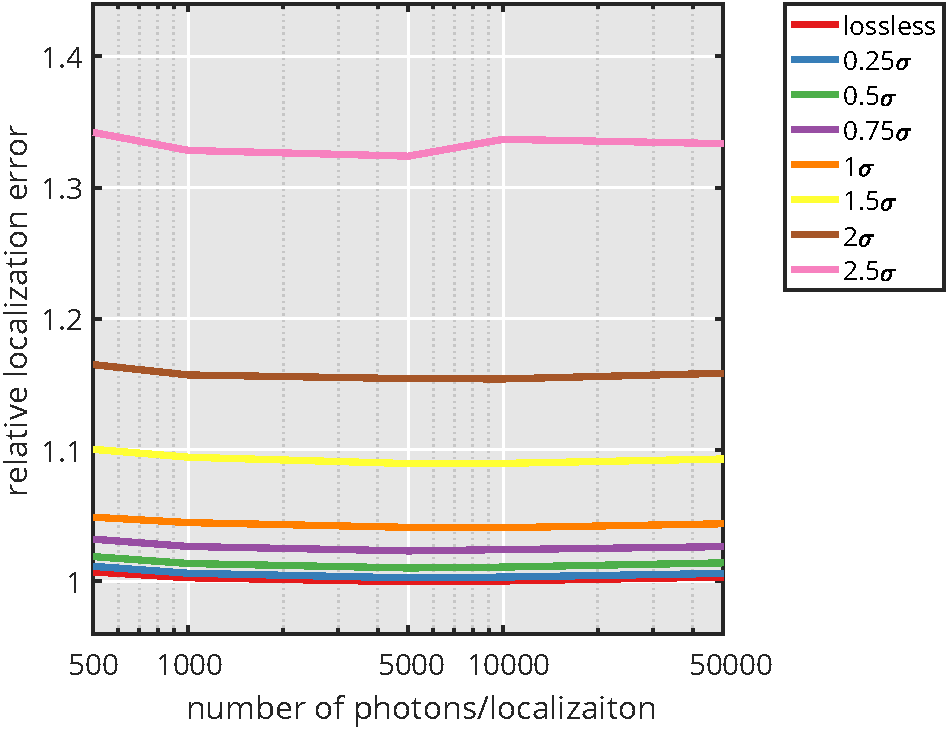
\includegraphics[page=1,width=0.5\textwidth]{SFig6_locprecVsNphotons}
      \bcaption[Change in localization error only depends on selected quantization step]{We simulated multiple datasets ( "\textbf{Supplementary Methods}") with different average photon numbers per localization. Background was kept at a constant average of 20 photons/pixel. Datasets were compressed at multiple compression levels (see legend), and localization error relative to the Cramér-Rao lower bound was calculated. The relative localization error only depends on the compression level, and not on the signal to background illumination ratio.}
      \label{fig:SFig6_locprecVsNphotons}
    \end{figure}

\section{Noise dependent lossy compression}

\section{Methods}
